% !TeX root = ../main.tex
\documentclass[../main.tex]{subfiles}
%\usepackage[subpreambles=true]{standalone}
%\usepackage{standalone}
%\usepackage{pgfplots}
%\pgfplotsset{compat=newest}
\begin{document}
\begin{figure}
\centering
%\includestandalone{sections/figures/2dplot}
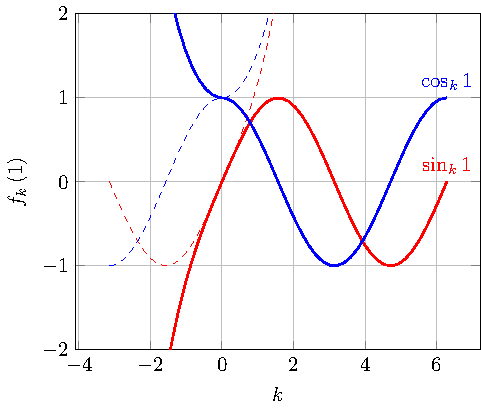
\includegraphics{sections/figures/2dplot.pdf}
\caption{Generalized trigonometric functions as function of $k$}\label{TrigonometryPlotted}
\figurenote{This graph shows the value of generalized trigonometric functions as solid line and trigonometric and hyperbolic functions in the unused domain as dashed line.}
\end{figure}
\begin{figure}
\centering
%\includestandalone{sections/figures/sine}
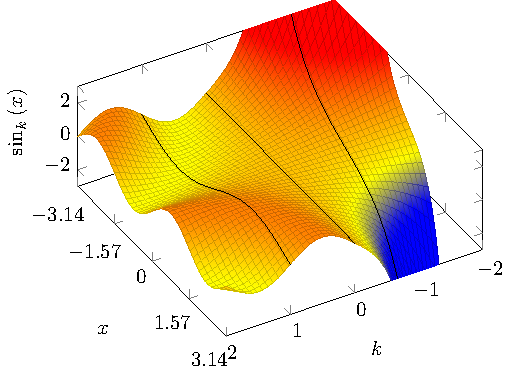
\includegraphics{sections/figures/sine.pdf}
\caption{Generalized sine function}\label{TrigonometrySinePlotted}
\end{figure}
\begin{figure}
\centering
%\includestandalone{sections/figures/sine_}
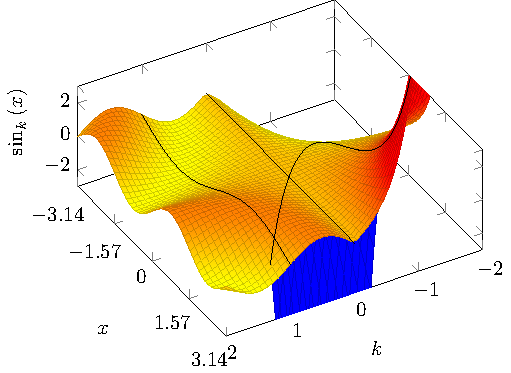
\includegraphics{sections/figures/sine_.pdf}
\caption{Generalized sine function variant}\label{TrigonometrySineVarPlotted}
\end{figure}
\begin{figure}
\centering
%\includestandalone{sections/figures/cosine}
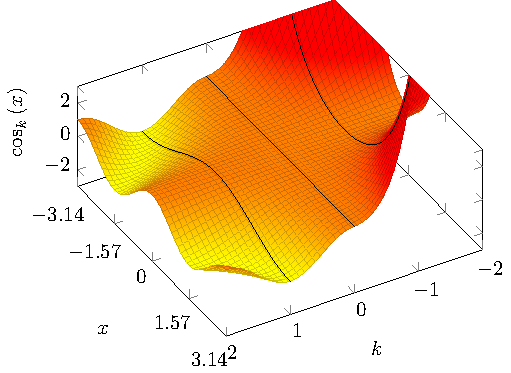
\includegraphics{sections/figures/cosine.pdf}
\caption{Generalized cosine function}\label{TrigonometryCosinePlotted}
\end{figure}
\end{document}